\chapter{Model i Druk 3D}
Jedym z głównych założeń projektu jaki powstał w ramach tej pracy (przedstawiony na rys. \ref{CAD_assembly}) była możliwość wydrukowania całej konstrukcji w 3D. Miało to na celu znaczne obniżenie kosztów produkcji, ale przede wszystkim umożliwienie znacznie szybszych przeróbek. Jest to o tyle istotne, że prowadzone będą badania z algorytami chodu - w przypdaku większości algorytmów wydłużenie pewnych elementów nogi może zmniejszyć wymagane prędkości ruchu serw. Eksperymenty takie mogą wymusić liczne przedruki poszczególnych członów nóg robota.\\

\begin{figure}[h!]
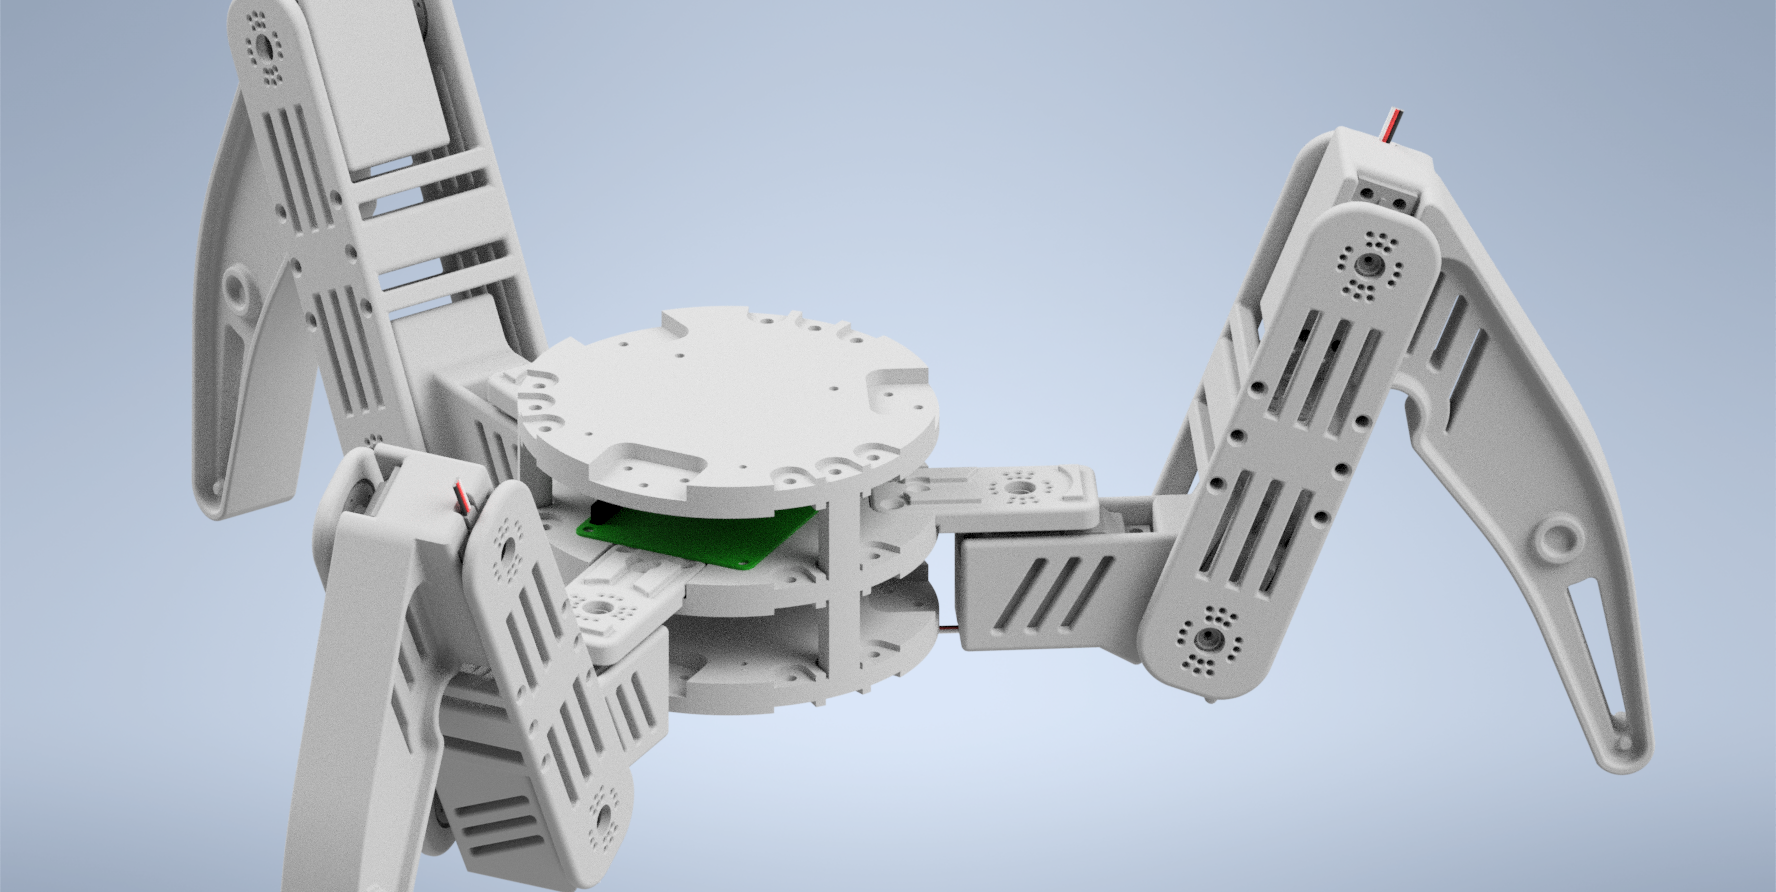
\includegraphics[width=\textwidth]{img/CAD_assembly.png}
\caption{Model złożeniowy.}
\label{CAD_assembly}
\end{figure}

Drugim założeniem projektowym jest modularność. Bardzo podobną modularność oferuje robot TurtleBot 3, który także był inspiracją stojącą za konstrukcją. Turtlebot składa się z wielu identycznych warstw, które zawierają liczne otwory montażowe umożliwiające przykręcenie w zasadzie dowolnego elemnentu. Projekt robiony w ramach tej pracy został oparty o podobną ideę. Także składa się z wielu identycznych warstw zawierających liczne otwory montażowe. Otwory te zostały dobrane pod kątem elektroniki jaka będzie montowana, ale na każdej z warstw można zamontować dowolny element w jednej z kilku konfiguracji.\\

Zostały także dokładnie zwymiarowane otwory montażowe znajdujące się na orczykach do zakupionych serw i przeniesione na poszczególne elementy nóg. Do montażu wspomnianych orczyków zakupione zostały śruby $M1.6$, co stanowi swojego rodzaju drobny eksperyment. Zwykle orczyki montuje się za pomocą kleju lub wkrętów dostarczanych wraz z serwomechanizmem. Są to jednak metody przynajmniej częściowo destrukcyjne - nie umożliwiają szybkiego demontażu i wymiany elementów, co jest bardzo ważnym elementem tego projektu. Zastosowanie śrub z nakrętkami rozwiązuje ten problem - jednak pojawia się pytanie czy nie generuje to innych problemów. Bardzo prawdopodobne jest pojawienie się problemu z samoodkręcającymi się śrubkami przy dłuższym użytkowaniu - zjawisko spowodowane drganiami generowanymi przez serwa. Było to już problemem w przypadku innych projektów - gdzie serwa odkręcały się od orczyków. Jednakże projekty tamte wykonane były w technologii CNC z blachy lub włókna węglowego - nigdy nie były drukowane w 3D. Bardzo możliwe jest że filament wytłumi drgania.

Projekt ten zawiera także pewną wadę konstrukcyjną - jest to bardzo cienki element łączący nogę z tułowiem (element nogi zero). Istnieje duże ryzyko gięcia a może nawet łamania się wyżej wymienionego elementu. Aby zmniejszyć to ryzyko, wspomniany element został miejscami pogrubiony. Dodatkowo, zakup metalowych orczyków także mógłby zmniejszyć ryzyko gięcia się konstrukcji. Najtrwalszym rozwiązaniem jednak byłoby stowrzenie dodatkowego elementu który byłby przytwierdzony do dolnej części obudowy i posiadałby oś obrotu z pierwszym elementem nogi -  "podtrzymywałby" ten elemnt od dołu.\\

Całość konstrukcji została zaprojektowana w programie Autodesk Inventor. Program ten został wybrany tylko i wyłącznie ze względu na fakt, że był autorowi projektu dość dobrze znany. Podczas projektowania należało także zdecydować się na pewne długości poszczególnych członów robota. Centralny okrąg został zaprojektowany na bazie RPi, można powiedzieć że jest to lekko powiększony okrąg opisany na prostokącie nakreślonym przez PCB Raspberry Pi. Długości członów nóg natomiast, zostały dobrane tak, aby przede wszystkim zmieściły się serwa i elementy nie obijały się o siebie podczas normalnej pracy. W tym miejscu, dla lepszej wizualizacji tworzonych modeli matematycznych, można także przenieść wymiary z rysunku \ref{math_model} na zaprojektowany model. Da to rysunek \ref{img:assembly_leg_lines}. Wykonanie projektu umożliwia także przypisanie konkretnych wartości do parametrów z rozdziału \ref{cha:math_model}. Przypisanie to jest widoczne w równaniu \ref{eq:physical_params}.

\begin{figure}[h!]
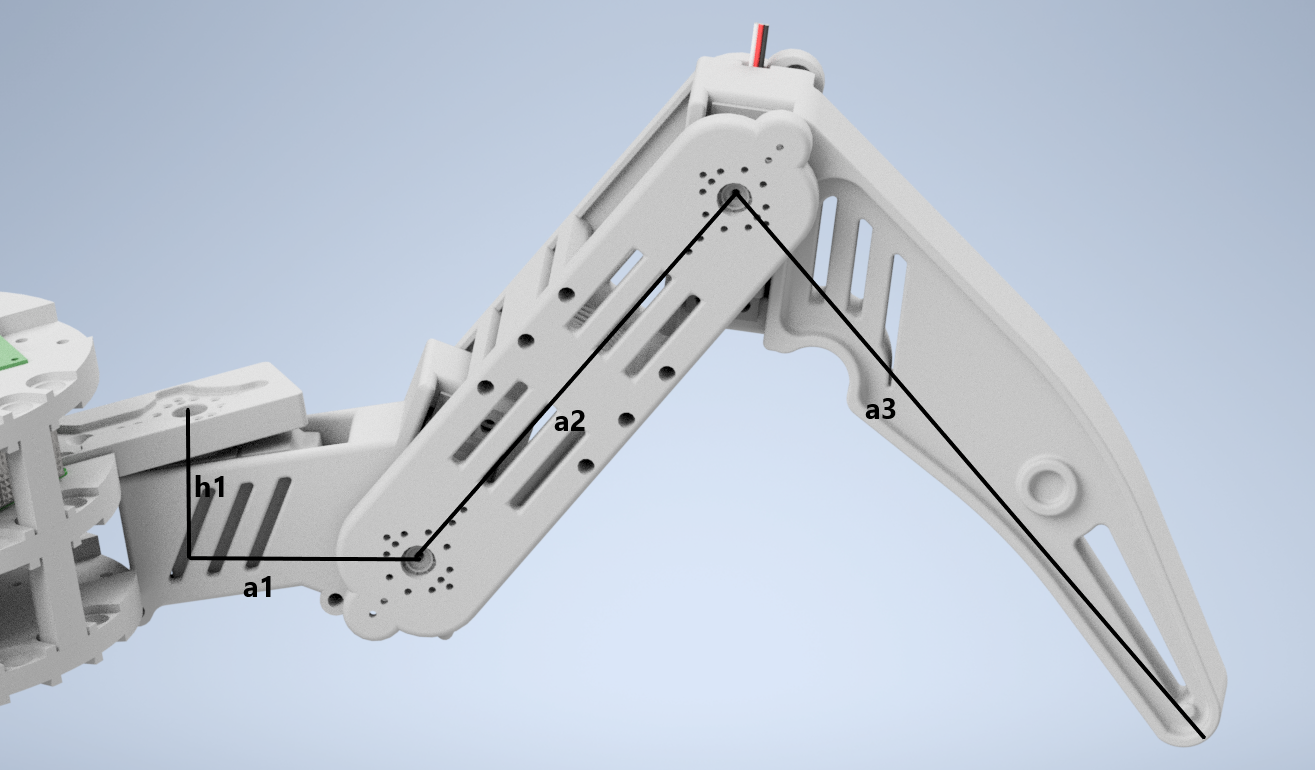
\includegraphics[width=\textwidth]{img/assembly_leg_lines.png}
\caption{Model złożeniowy pojedynczej nogi z naniesionymi wymiarami.}
\label{img:assembly_leg_lines}
\end{figure}

\begin{equation} \label{eq:physical_params}
\begin{split}
    h_1 &= 40\\
    a_1 &= 55\\
    a_2 &= 125\\
    a_3 &= 180\\
\end{split}
\end{equation}

Modele zostały wydrukowane na drukarce Zortrax M200. Została ona wybrana ze względu na jej dostępnośc na uczelni. Dodatkowo, aby przygotować pliki pod druk, należało model przetworzyć programem Z-Suite. W programie większość ustawień pozostawiana była bez zmian, jedynie dwa istotne ustawienia zostały dostosowane do projektu. Zostało ustawione minimalne, niezerowe wypełnienie, około $10\%$ . Warstwy wierzchnia i spodnia zostały ustawione na najgrubszą możliwą opcję. Ustawienia te znalezione zostały eksperymentalnie - wydają się najlepiej balansować między wytrzymałością a czasem druku i ilością zużytego materiału. Dodatkowo, przed ostatecznym wydrukiem, zwiększone zostały o około $0.3-0.4 mm$ wszystkie otwory montażowe. Modele podczas druku "puchną" i w pierwszych wydrukach otwory te były znacznie mniejsze niż na tworzonych szkicach.\\
